\documentclass[11pt]{article}
\usepackage{header}
\def\title{HW 05}

\begin{document}
\maketitle
\fontsize{12}{15}\selectfont

\begin{center}
    Due: Saturday, 10/5, 4:00 PM \\
    Grace period until Saturday, 10/5, 6:00 PM \\
\end{center}

\section*{Sundry}
Before you start writing your final homework submission, state briefly how you worked on it.  Who else did you work with?  List names and email addresses.  (In case of homework party, you can just describe the group.)

\begin{solution}
  I worked with Lawrence Rhee (lawrencejrhee@berkeley.edu). 
  We discussed our approaches to each problem and asked each other questions.  
\end{solution}
\vspace{15pt}

\Question{RSA Practice}

\notelinks{\href{https://www.eecs70.org/assets/pdf/notes/n7.pdf}{Note 7}}
Consider the following RSA scheme and answer the specified questions.
\begin{Parts}
 
    \Part Assume for an RSA scheme we pick $2$ primes $p = 5$ and $q = 11$ with encryption key $e = 9$, what is the decryption key $d$? Calculate the exact value.
    
    
    \Part If the receiver gets 4, what was the original message? \label{easy-rsa-b}
    
    
    \Part Encode your answer from part (\ref{easy-rsa-b}) to check its correctness.
    
\end{Parts}

\begin{solution} \begin{Parts} \Part 
By the RSA scheme, we have that $d$ is the inverse of $e$ in mod $(p-1)(q-1)$.
$(p-1)(q-1)=40$ and $e=9$. We can see that $9*9=81\equiv1\pmod{40}$. Thus, $d=9$.

\Part 
By the RSA scheme, the original message is $y^d\pmod{N}$.
We calculate that $N=pq=55$. 
$4^9\equiv64^3\equiv9^3\equiv14\pmod{55}$. Thus, original message $x=14$.

\Part 
By the RSA scheme, the encoded message is $x^e\pmod{N}$. 
Then we have that $14^9\equiv4\pmod{55}$. 
Thus, we verify that the encoded message is 4 as stated in part (b).

\end{Parts}\end{solution}\newpage

\Question{Tweaking RSA}

\notelinks{\href{https://www.eecs70.org/assets/pdf/notes/n7.pdf}{Note 7}}
You are trying to send a message to your friend, and as usual, Eve is trying to decipher what the message is.
  However, you get lazy, so you use $N = p$, and $p$ is prime.
  Similar to the original method, for any message $x \in \{0,1, \ldots, N-1\}$, $E(x) \equiv x^e$ (mod $N$), and $D(y) \equiv y^d$ (mod $N$).
\begin{Parts}
  \Part
  Show how you choose $e$ and $d$ in the encryption and decryption function, respectively. Prove the correctness property: the message $x$ is recovered after it goes through your new encryption and decryption functions, $E(x)$ and $D(y)$.

    \Part
    Can Eve now compute $d$ in the decryption function? If so, by what algorithm?

    \Part Now you wonder if you can modify the RSA encryption method to work with three primes ($N = pqr$ where $p, q, r$ are all prime). Explain the modifications made to encryption and decryption and include a proof of correctness showing that $D(E(x)) = x$.

\end{Parts}
\begin{solution}\begin{Parts}\Part 
Choose some $e$ that is coprime to $p-1$. 
Then there exists a modular inverse. 
Find $d$ so that $de\equiv1\pmod{p-1}$.
Then, for any message $x\pmod{p}$ 
we can write $x^{ed}$ as $x^{k(p-1)+1}$ for some integer $k$.
By FLT, we have that $x^{p-1}\equiv1\pmod{p}$.
Thus, $x^{ed}\equiv x\pmod{p}$ for all $x$.

\Part Eve knows $(N=p, e)$, and about the scheme you are using.
She can easily find the inverse $d$ of $e$ $\pmod{p-1}$ via extended GCD algorithm (which runs ~logarithmic time).
Now, Eve can snoop all your packets and you aren't secure!

\Part 
Claim: we can work successfully with 3 primes, 
by choosing $e$ so that $e$ is relatively prime to $(p-1)(q-1)(r-1)$
and finding $d$ so that $de\equiv1\pmod{(p-1)(q-1)(r-1)}$.

Proof: Suppose $ed\equiv1\pmod{(p-1)(q-1)(r-1)}$.
Then $x^{ed}-x$ can be written as 
$$x^{k(p-1)(q-1)(r-1)+1}-x$$
for some integer $k$.
Factoring out $x$ we rewrite:
$$x(x^{k(p-1)(q-1)(r-1)}-1)$$
Case 1: suppose $x$ is a multiple of $p$. Then, $x^{ed}-x$ is a multiple of $p$.
\\Case 2: suppose $x$ is not a multiple of $p$. 
Then, by FLT we have that $x^{p-1}\equiv1\pmod{p}$.
Then the equation is equivalent to $x(1-1)\equiv0\pmod{p}$.
Then, $x^{ed}-x$ is a multiple of $p$.
\\Then, no matter what $x$ we choose, $x^{ed}-x$ is a multiple of $p$.
Similarly, doing the same process over $q$ and $r$, we have that $x^{ed}-x$ is a multiple of $q$ and $r$ as well.
Then, $x^{ed}-x\equiv0\pmod{pqr}$
Thus, $x^{ed}\equiv x\pmod{pqr}$ for all $x$ as desired.
\end{Parts}\end{solution}\newpage

\Question{Trust No One}

\notelinks{\href{https://www.eecs70.org/assets/pdf/notes/n8.pdf}{Note 8}}
Gandalf has assembled a fellowship of nine peoples to transport the One Ring to the fires of Mount Doom: five humans, two hobbits, one elf, and one dwarf. The ring has great power that may be of use to the fellowship during their long and dangerous journey. Unfortunately, the use of its immense power will eventually corrupt the user, so it must not be used except in the most dire of circumstances. To safeguard against this possibility, Gandalf wishes to keep the instructions a secret from members of the fellowship. The secret must only be revealed if enough members of the fellowship are present and agree to use it.

Gandalf has hired your services to help him come up with a secret sharing scheme that accomplishes this task, summarized by the following points:
\begin{itemize}

\item There is a party of five humans, two hobbits, an elf, and a dwarf, and a secret message that must remain unknown to everyone if not enough members of the party agree.
\item A group of people consisting of at least two people from different people classes and at least one people class that is fully represented (i.e., has all members present) can unlock the secret of the ring.

\end{itemize}

A few examples: only five humans agreeing to use the ring is not enough to know the instructions. One hobbit and four humans is not enough. However, all five humans and one hobbit agreeing is enough. Both hobbits and the dwarf agreeing is enough.

\begin{solution}
Let s be the secret number. 
Generate 4 random polynomials and distribute information as follows: 
\\U(x) with degree 5 so that U(0) = s. Index the humans from 1 to 5. Give human i the pair (i, U(i)). Give the pair (6, U(6)) to every non-human.
\\O(x) with degree 2 so that O(0) = s. Index the hobbits from 1 to 2. Give hobbit i the pair (i, O(i)). Give the pair (3, O(3)) to every non-hobbit.
\\E(x) with degree 1 so that E(0) = s. Give the singular elf the pair (1, E(1)). Give the pair (2, E(2)) to every non-elf.
\\D(x) with degree 1 so that D(0) = s. Give the singular dwarf the pair (1, D(1)). Give the pair (2, D(2)) to every non-dwarf.
\\Then, it follows, to reconstruct any of these polynomials,
you must have the class corresponding to that polynomial all together sharing their pairs
and any 1 being outside of the class sharing their pair, in order to have enough information.
Then, once you reconstructed any of these 4 polynomials, evaluating it at 0 gives you the secret.
Having partial information of any of these polynomials doesn't tell you anything about any of the other polynomials or $s$ itself.
\end{solution}\newpage

\Question{Equivalent Polynomials}

\notelinks{\href{https://www.eecs70.org/assets/pdf/notes/n7.pdf}{Note 7},\href{https://www.eecs70.org/assets/pdf/notes/n8.pdf}{Note 8}}
This problem is about polynomials with coefficients in $\text{GF}(p)$ for some prime $p \in \mathbb{N}$. We say that two such polynomials $f$ and $g$ are \emph{equivalent} if $f(x) \equiv g(x) \pmod{p}$ for every $x \in \text{GF}(p)$. 

\begin{Parts}
    \Part Show that $f(x)=x^{p-1}$ and $g(x)=1$ are \textbf{not} equivalent polynomials under $\text{GF}(p).$

    \Part Use Fermat's Little Theorem to find a polynomial with degree strictly less than 5 that is equivalent to $f(x) = x^5$ over $\text{GF}(5)$; then find a polynomial with degree strictly less than 11 that is equivalent to $g(x) = 4x^{70} + 9x^{11} + 3$ over $\text{GF}(11)$.

    \Part In $\mathrm{GF}(p)$, prove that whenever $f(x)$ has degree $\ge p$, it is equivalent to some polynomial $\tilde f(x)$ with degree $< p$.
\end{Parts}

\begin{solution}\begin{Parts}\Part 
  Suppose $x=0$. Then $f(0)=0^{p-1}=0\neq g(0)=1$.
  Thus, they are NOT equivalent polynomials under GF(p), 
  since it does not satisfy they are equivalent for EVERY $x\in GF(p)$.
  
\Part 
By FLT, for all $x\in{1,...,p-1}$: $x^4\equiv 1\pmod{5}$.
Multiplying both sides by $x$, we have that $x^5\equiv x\pmod{5}$, 
which still satisfies that $x^4\equiv 1\pmod{5}$ for non-zero $x$.
However, unlike the previous equation, when $x=0$, both sides are 0 and equal.
Therefore, for all $x\in GF(5)$, we have that $x^5=x$. 
Thus, the polynomial $p(x)=x$ is equivalent to $f(x)=x^5$.
\\For the second part, we have (similarly) that
$$x^{70}\equiv x^{10}\pmod{11}$$
and
$$x^{11}\equiv x^1\pmod{11}$$
This is because if $x$ is 0 both sides are equal to 0
and if $x$ is not zero, both sides are equal due to FLT (in both equations). 
Then, we have a polynomial $p(x)=4x^{10}+9x+3$ that is equivalent to $g(x)$.

\Part 
Let some power of $x: x^k$ exist in $f(x)$ so that $k\geq p$.
Then, $k\geq(p-1)+1$
Then, $k$ can be written as $k(p-1)+r$ for some positive integer $k$ and integer $r=0,\dots,p-2$.
\\Suppose $r$ is non-zero. 
Then, by our discoveries from (a) and (b), we have it that $x^k\equiv x^r\pmod{p}$.
\\Suppose $r$ is zero. 
Then, by our discoveries from (a) and (b), we have it that $x^k\equiv x^{p-1}\pmod{p}$. 
\\Then all $x^k$ can be replaced with $x^n$ so that $n\in{0,...,p-1}$.
After all the replacements, we are left with a polynomial $f'(x)$ so that all powers of $x$ are less than $p$.
This is a polynomial with degree < $p$ by definition, thus we are done.
\end{Parts}\end{solution}\newpage

\Question {Lagrange?  More like Lamegrange.}  
\notelinks{\href{https://www.eecs70.org/assets/pdf/notes/n8.pdf}{Note 8}}
In this problem, we walk you through an alternative to Lagrange interpolation.

\begin{Parts}

	\Part Let's say we wanted to interpolate a polynomial through a single point, $(x_0, y_0)$.  What would be the polynomial that we would get?  (This is not a trick question. A degree 0 polynomial is fine.)
	
	\Part Call the polynomial from the previous part $f_0(x)$.  Now say we wanted to define the polynomial $f_1(x)$ that passes through the points $(x_0, y_0)$ and $(x_1, y_1)$.  If we write $f_1(x) = f_0(x) + a_1(x - x_0)$, what value of $a_1$ causes $f_1(x)$ to pass through the desired points?
	
	\Part Now say we want a polynomial $f_2(x)$ that passes through $(x_0, y_0)$, $(x_1, y_1)$, and $(x_2, y_2)$.  If we write $f_2(x) = f_1(x) + a_2(x - x_0)(x - x_1)$, what value of $a_2$ gives us the desired polynomial?
	
	\Part Suppose we have a polynomial $f_i(x)$ that passes through the points $(x_0, y_0)$, ..., $(x_i, y_i)$ and we want to find a polynomial $f_{i + 1}(x)$ that passes through all those points and also $(x_{i + 1}, y_{i + 1})$.  If we define $f_{i + 1}(x) = f_i(x) + a_{i + 1}\prod_{j = 0}^i (x - x_j)$, what value must $a_{i + 1}$ take on?
	
	
\end{Parts}
\begin{solution}\begin{Parts}\Part 
$f_0=y_0$

\Part 
$$f_1(x)=f_0(x)+a_1(x-x_0)$$
Clearly, when $x_0$ is plugged into this equation, it works. 
$f_0(x)$ evaluates it as desired, and the term with the coefficient evaluates it to 0.
So we only have to find a coefficient that works in with the new point $(x_1,y_1)$.
$$f_1(x_1)=f_0(x_1)+a_1(x_1-x_0)=y_1$$
$$a_1=\frac{y_1-f_0(x_1)}{x_1-x_0}$$
(You could further simplify this to $\frac{y_1-y_0}{x_1-x_0}$)

\Part
Similarly:
$$f_2(x)=f_1(x)+a_2(x-x_0)(x-x_1)$$
All the points before $(x_2,y_2)$ work, and we only worry about finding a coefficient that works in with $(x_2,y_2)$.
$$f_2(x_2)=f_1(x_2)+a_2(x_2-x_0)(x_2-x_1)=y_2$$
$$a_2=\frac{y_2-f_1(x_2)}{(x_2-x_0)(x_2-x_1)}$$

\Part 
Now to generalize this:
$$a_{i+1}=\frac{y_{i+1}-f_i(x_{i+1})}{\prod_{j=0}^i(x_{i+1}-x_j)}$$ 
The mundane and trivial proof, similar to that of (c), is left to the reader.
(Just kidding, see the next image below).
\begin{figure}[H]\centering
  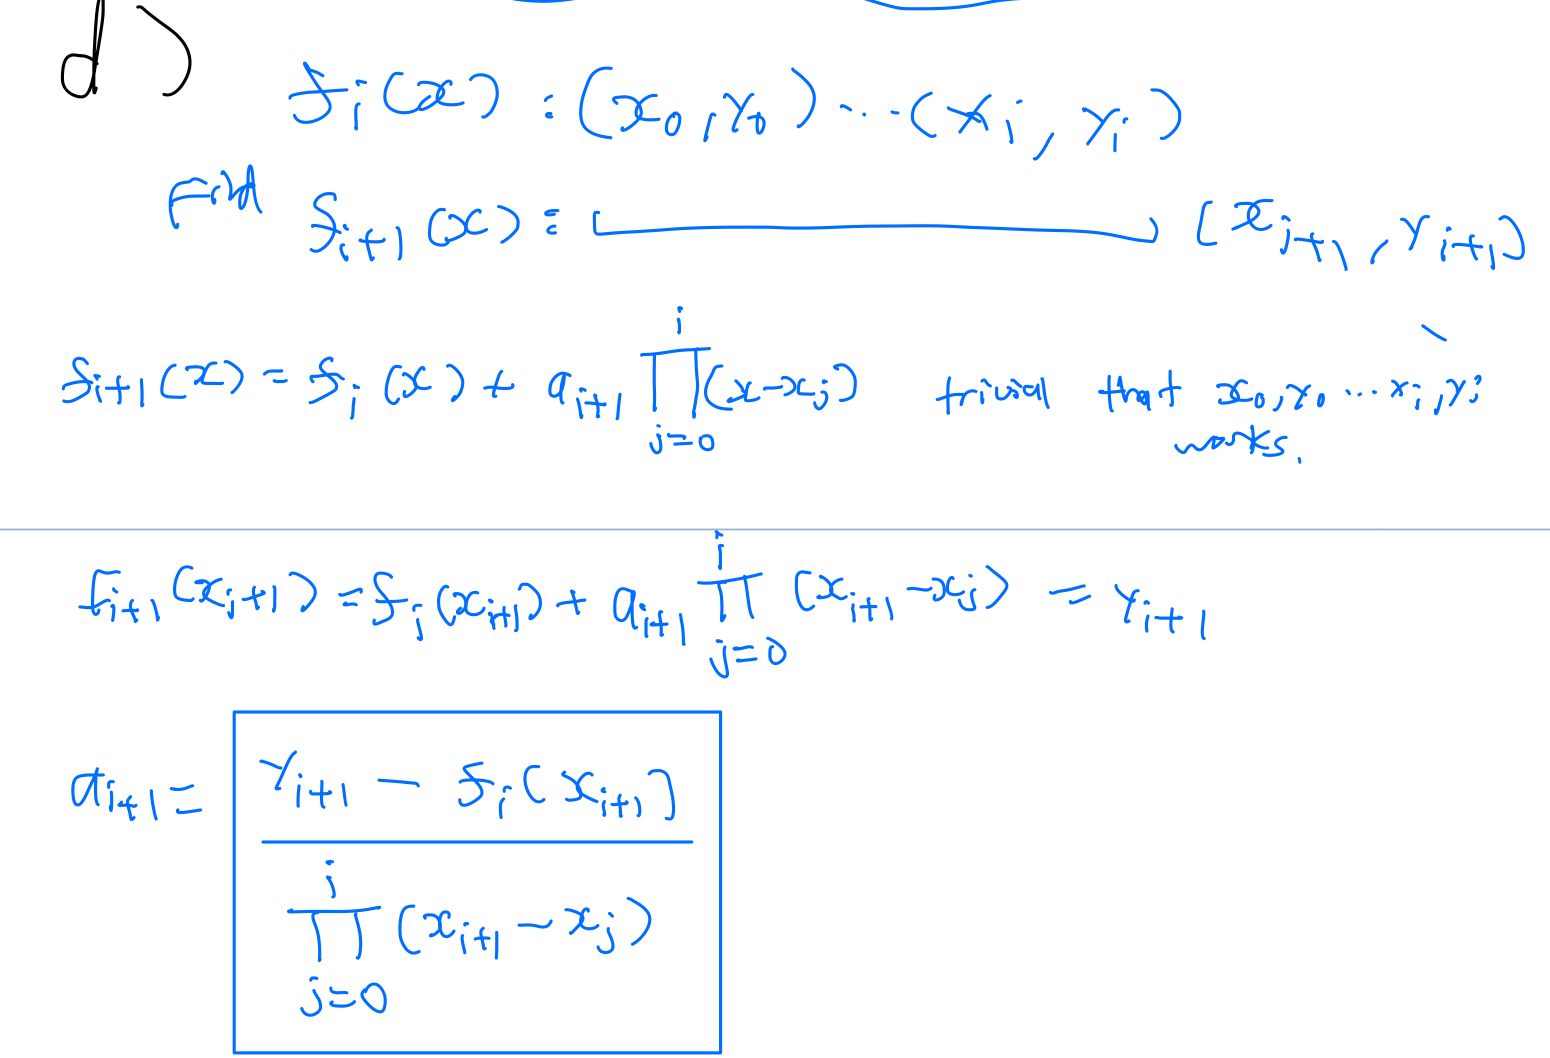
\includegraphics[width=0.8\linewidth]{assets/IMG_3283.jpg}
\end{figure}
\end{Parts}\end{solution}

\end{document}

\begin{comment}
Generate a random polynomial P(X) with degree 1 so that P(0)=s.
Generate 4 random polynomials: 
U(x) with degree 4 so that U(0) = P(1), 
O(x) with degree 1 so that O(0) = P(2), 
E(x) with degree 0 so that E(0) = P(3), 
D(x) with degree 0 so that D(0) = P(4).
For $i=1,\dots,5$: human i gets a tuple: (1, i, U(i)).
For $i=1,2$: hobbit i gets a tuple: (2, i, O(i)).
The singular elf gets a tuple: (3, 1, E(1)).
The singular dwarf gets a tuple: (4, 1, D(1)).
Then, in order to find the secret P(0), 2 class
\end{comment}